\documentclass[a4paper,12pt]{article}

\usepackage{amsmath,amsfonts,mathtools}
\usepackage{amsthm}
\usepackage{graphicx}
\usepackage{hyperref}
\usepackage{enumitem}

% For displaying code
\usepackage{listings}
\usepackage{color}

\definecolor{dkgreen}{rgb}{0,0.6,0}
\definecolor{gray}{rgb}{0.5,0.5,0.5}
\definecolor{mauve}{rgb}{0.58,0,0.82}

% Settings for displaying code
\lstset{frame=tb,
  language=Python,
  aboveskip=3mm,
  belowskip=3mm,
  showstringspaces=false,
  columns=flexible,
  basicstyle={\small\ttfamily},
  numbers=none,
  numberstyle=\tiny\color{gray},
  keywordstyle=\color{blue},
  commentstyle=\color{dkgreen},
  stringstyle=\color{mauve},
  breaklines=true,
  breakatwhitespace=true,
  tabsize=3
}

% Personal definitions
\newcommand{\lra}{\ensuremath{\longrightarrow{}}}
\newcommand{\vect}[1]{\mathbf{#1}}
\renewcommand{\qedsymbol}{\rule{0.7em}{0.7em}}

% Theorem commands
\newtheorem{lem}{Lemma}
\newtheorem{thm}{Theorem}
\newtheorem{defn}{Definition}

% Set spacing
\setenumerate{itemsep=1.5pt,parsep=1.5pt,topsep=0.5pt}
\setlist{itemsep=1.5pt,parsep=1.5pt,leftmargin=1pt}
\setitemize{itemsep=1.5pt,parsep=1.5pt,topsep=0.5pt}

% set 1" margins on 8.5" x 11" paper
% top left is measured from 1", 1"
\topmargin       0in
\oddsidemargin   0in
\evensidemargin  0in
\headheight      0in
\headsep         0in
\topskip         0in
\textheight      9in
\textwidth       6.5in

\begin{document}
\title{General ConvNet Notes}
\author{Sean Wu}
\date{\today}
\maketitle

\tableofcontents

\pagebreak

% set spacing
\setlength{\parindent}{0em}
\setlength{\parskip}{1em}

\section{ConvNet Structure}

\subsection{ConvNet Layers}
\begin{description}
  \item[Convolutional Neural Net (ConvNet):] specialized neural nets
\end{description}
\begin{itemize}
  \item Explicitly assume that inputs are images (reduces params req)
  \item Regular neural nets don't scale well w/ images because they maintain full connectivity for all neurons $\implies$ many parameters and overfitting
  \item ConvNets have layers w/ neurons called \textbf{activation volumes} arranged in 3 dimensions (\textbf{length}, \textbf{height}, \textbf{depth})
  \item Each layer transforms an input 3D volume to an output 3D volume w/ some differentiable function that may/may not have parameters
  \item ConvNets transform image layer by layer
  \item Params are trained w/ gradient descent so class scores that the ConvNet computes are consistent w/ training labels
\end{itemize}

\begin{figure}[th]
  \centering
  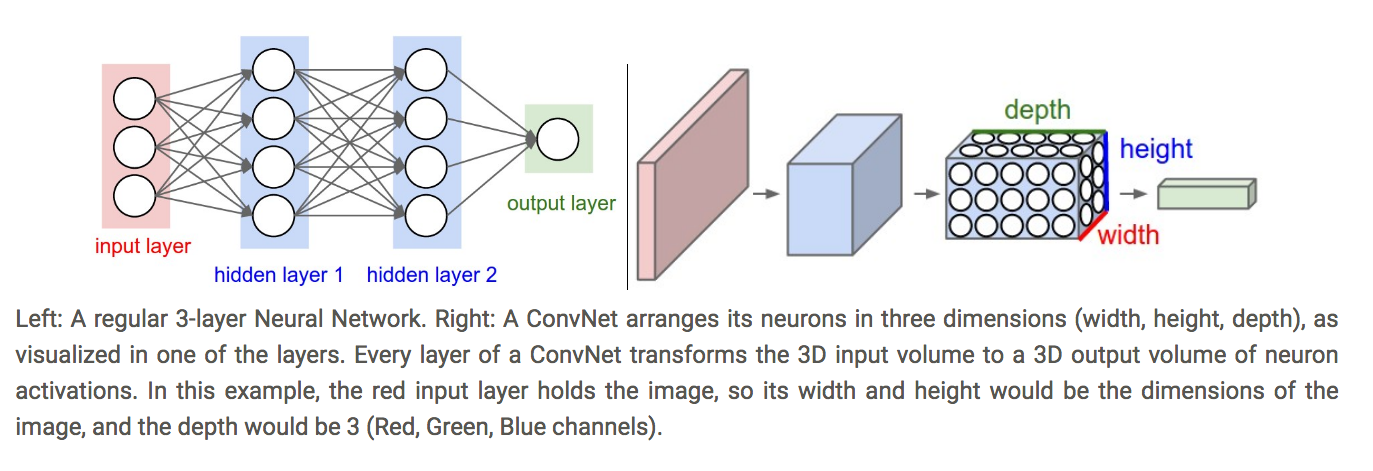
\includegraphics[width=165mm, scale=1]{images/ConvNet-Volumes.png}
  \caption{Illustration of ConvNet layers as Volumes}
  \label{Volumes}
\end{figure}


\subsection{Main ConvNet Layer Types}
\begin{enumerate}
  \item Convolutional Layer (CONV)
  \item Pooling Layer (POOL)
  \item Fully-Connected Layer (FC)
\end{enumerate}
\begin{itemize}
  \item CONV/FC/POOL have hyperparameters, RELU doesn't
\end{itemize}


\subsection{Example ConvNet Architecture}
\begin{itemize}
  \item Ex. ConvNet for CIFAR-10 classification
  \item INPUT \lra CONV \lra RELU \lra POOL \lra FC
\end{itemize}
\begin{enumerate}
    \item \textbf{INPUT} ($32\times 32\times 3$): takes raw pixel values of $32\times 32$ RGB image
    \item \textbf{CONV} ($32\times 32\times 12$ if using 12 filters): computes output of neurons connected to input w/ dot product betw their weights and the filter
    \item \textbf{RELU} ($32\times 32\times 12$): applies elementwise activation function (ex. $f(x) = max(0,x)$)
    \item \textbf{POOL} ($16\times 16\times 12$): downsamples along width \& height (depth unchanged)
    \item \textbf{FC} ($1\times 1\times 10$): computes class scores (1 neuron per class score)
\end{enumerate}

\begin{figure}[th]
  \centering
  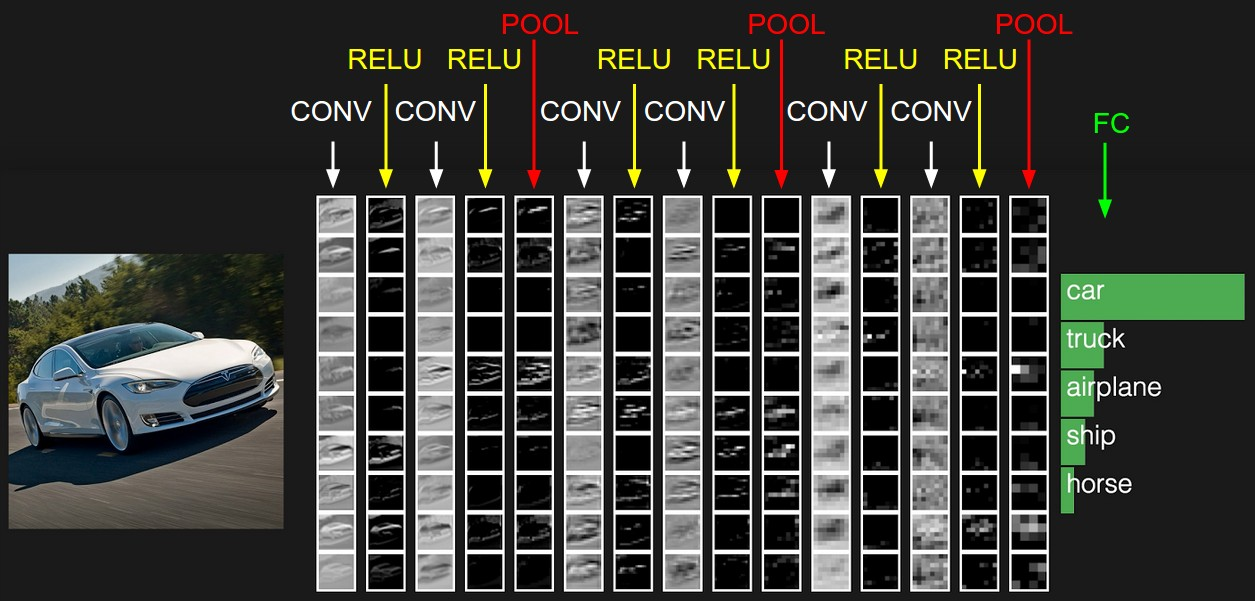
\includegraphics[width=165mm, scale=1]{images/ConvNet-Example.jpeg}
  \caption{Illustration of ConvNet layers as Volumes}
  \label{Example}
\end{figure}


\subsection{Convolutional Layer (CONV)}
\begin{itemize}
  \item Input Volume: $W_1\times H_1\times D_1$
  \item Consists of filters that are convolved across width and height of input volume during forward pass
  \begin{itemize}
    \item Computes dot product betw entries of filter and input at any position
    \item Produces 2D activation maps that are stacked along depth dimension that give responses of a filter at each any position
  \end{itemize}
  \item Helps ConvNet learn filters that activate when some type of visual feature is detected (ex. edge, specific colour, etc)
  \item Requires 4 hyperparams
  \begin{enumerate}
    \item \# of filters, \textbf{K}
    \item Spatial extent (size of filter), \textbf{F}
    \item Stride (distance betw centres of filters), \textbf{S}
    \item Zero padding, \textbf{P}
  \end{enumerate}
  \item Output Volume: $W_2\times H_2\times D_2$
\end{itemize}

\textbf{Output Volume Equations}
\begin{align}
  W_2 &= (W_1 - F + 2P)/S + 1 \\
  H_2 &= (H_1 - F + 2P)/S + 1 \\
  D_2 &= K
\end{align}


\begin{itemize}
  \item With parameter sharing, the CONV introduces $F\cdot F\cdot D_1$ weights per filter for a total of $(F\cdot F\cdot D_1)\cdot K$ weights and K baises
  \item In output volume, the d-th slice ($W_2\cdot H_2$) is result of convolution of d-th filter over input volume w/ stride S and then offset by dth biases
\end{itemize}
\begin{description}
  \item[Common Hyperparameter Settings:] $F = 3$, $S = 1$, $P = 1$
\end{description}

\begin{description}
  \item[Receptive field (filter):] hyperparameter representing spatial extent of connectivity of each neuron to a local region of input volume
\end{description}
\begin{itemize}
  \item Extent of connectivity along depth axis equals depth of input volumes
\end{itemize}

\begin{figure}[th]
  \centering
  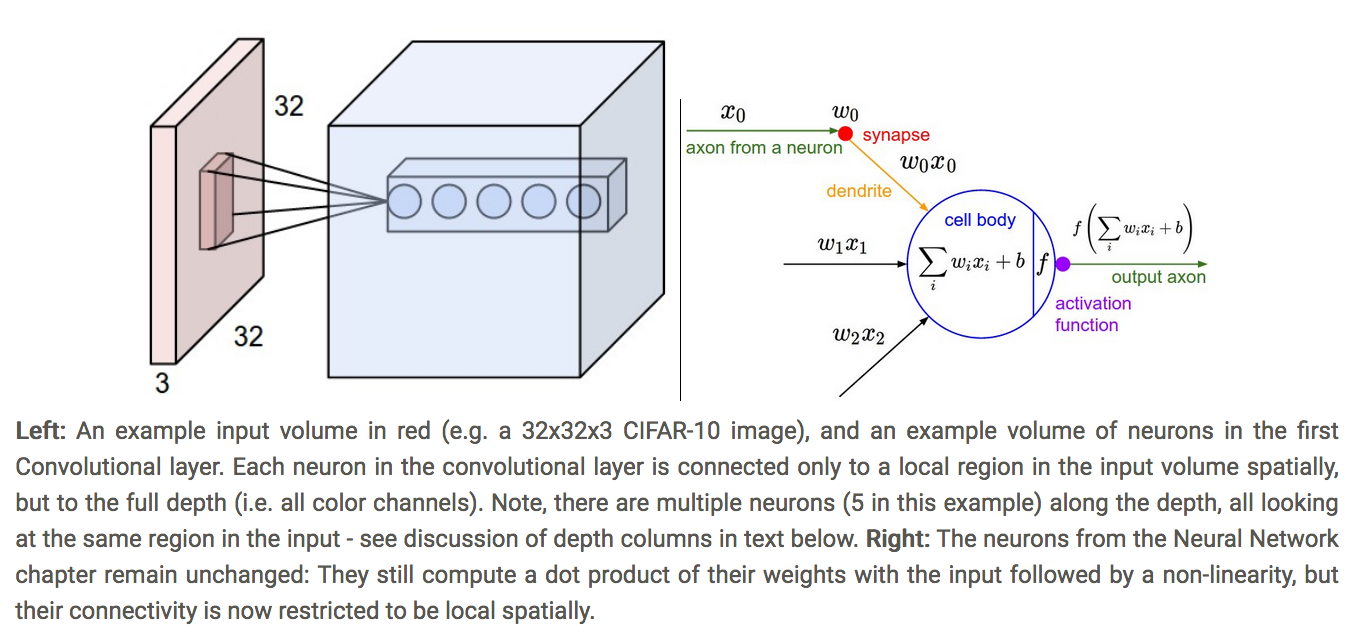
\includegraphics[width=165mm, scale=1]{images/ConvNet-Filter-Weights.png}
  \caption{Illustration of ConvNet layers as Volumes}
  \label{Filter-Weights}
\end{figure}

\subsection{Spatial Arrangement of CONV Neurons}
\begin{itemize}
  \item 3 hyperparameters control size of output volume
\end{itemize}
\begin{enumerate}
  \item Depth (equivalent to \# of filters, $D$)
  \item Stride ($S$)
  \item Zero-padding ($P$)
\end{enumerate}

\begin{description}
  \item[Depth:] corresponds to \# of filters
\end{description}
\begin{itemize}
  \item Each filter learns to look for something different in the input
\end{itemize}
\begin{description}
  \item[Depth column:] set of neurons that are all looking at the same region of the input
  \item[Stride] Speed at which filter is moved
\end{description}
\begin{itemize}
  \item Stride of $S = 1$ moves filters 1 pixel at a time
  \item Larger strides produce smaller output volumes spatially
\end{itemize}
\begin{itemize}
  \item Note: stride is constrained by $W$, $F$, $P$ since $(W - F + 2P)/S$ must be an integer
  \item Otherwise, neurons don't fit symmetrically across input
  \item Considered invalid setting of hyperparameters and ConvNet library could throw exception, zero pad, or crop to make it fit
\end{itemize}
\begin{itemize}
  \item If stride is $S=1$, usually set zero padding as $P=(F-1)/2$ so input and output volume have same size
\end{itemize}

\subsection{Parameter Sharing}
\begin{itemize}
  \item Parameter sharing is used in CONV to reduce \# of params
  \item Assumes if a feature is useful to computer at some spatial position $(x,y)$ then it should also be useful to compute it at a different position $(x_2, y_2)$
  \item i.e. denote a single 2D slice of depth as a \textbf{depth slice} and set its neurons to use the same weights and biases (1 depth slice per filter)
  \item Thus CONV layer will only have 1 weight per depth slice
  \item During backpropagation, the gradient for every neuron's weights are added up across each depth slice but only a single set of weights is updated per slice
  \item ex. a $55\times 55\times 96$ input has 96 depth slices ($55\times 55$) and uses only 96 unique weights
  \item Note: if all neurons in a single depth slice use the same weight vector, the forward pass of CONV layer in each depth slice can be computed as a \textbf{convolution} of neurons weights w/ input volume
  \item Usually refer to the sets of weights as a \textbf{filter} or \textbf{kernel} that is convolved w/ input
\end{itemize}
\begin{itemize}
  \item Param sharing does not work when we expect completely diff features on each side of input image
  \item Use less strict param sharing scheme (called  a \textbf{locally-connected layer})
\end{itemize}

\subsubsection{Numpy Examples}
\begin{itemize}
  \item Input volume: numpy array \lstinline{X}
  \item Depth column at position $(x,y)$: \lstinline{X[x,y,:]}
  \item Depth slice/activation map at depth $d$: \lstinline{X[:,:,d]}
\end{itemize}
\begin{itemize}
  \item ex. input volume \lstinline{X} has shape \lstinline{X.shape: (11,11,14)} and uses zero padding $P=0$, filter size $F=5$, and stride $S=2$
  \item Output volume has size: $(11-5)/2 + 1 = 4$ giving volume width \& height of 4
\end{itemize}

\begin{lstlisting}
# First activation map in output volume V w/ parameter sharing
# W0 is the neuron's weight vector and b0 is the bias
# Dimensions along width are increasing in steps of 2 (stride)
# Each line rep dot product of 1 channel of image multiplied by filter W0
V[0,0,0] = np.sum(X[:5,:5,:]) * W0) + b0
V[1,0,0] = np.sum(X[2:7,:5,:] * W0) + b0
V[2,0,0] = np.sum(X[4:9,:5,:] * W0) + b0
V[3,0,0] = np.sum(X[6:11,:5,:] * W0) + b0
\end{lstlisting}

\begin{itemize}
  \item Note: \lstinline{*} in numpy means elementwise multiplication
\end{itemize}

\begin{lstlisting}
# Second activation map in output volume V w/ parameter sharing
# Note: Some steps (including activation functions like ReLU) are not shown
V[0,0,1] = np.sum(X[:5,:5,:] * W1) + b1
V[1,0,1] = np.sum(X[2:7,:5,:] * W1) + b1
V[2,0,1] = np.sum(X[4:9,:5,:] * W1) + b1
V[3,0,1] = np.sum(X[6:11,:5,:] * W1) + b1
V[0,1,1] = np.sum(X[:5,2:7,:] * W1) + b1 #(example of going along y)
V[2,3,1] = np.sum(X[4:9,6:11,:] * W1) + b1 #(or along both)
\end{lstlisting}

\pagebreak

\begin{figure}[th]
  \centering
  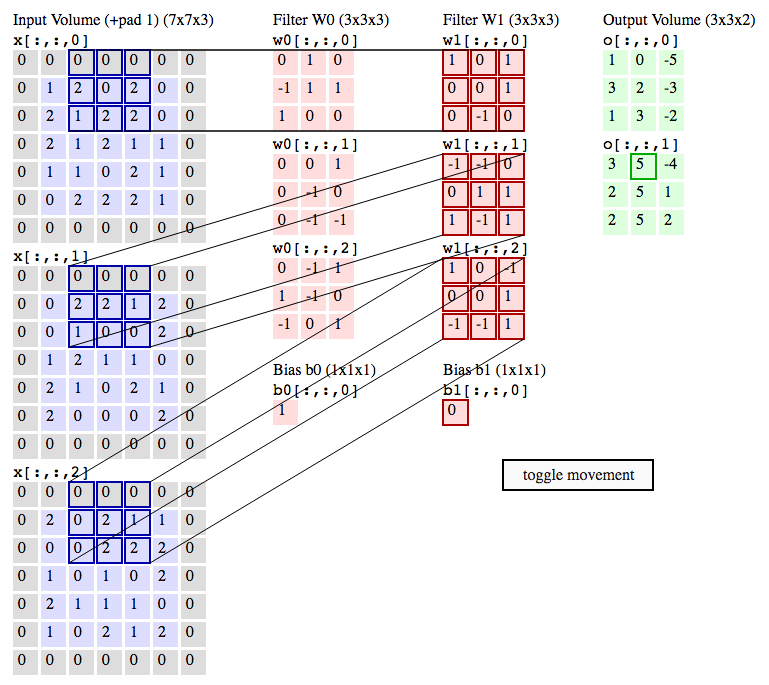
\includegraphics[width=165mm, scale=1]{images/Convolution-Visualization.png}
  \caption{Visualization of above numpy code for convolutions}
  \label{Visualization}
\end{figure}


\section{Convolutions as Matrix Multiplication}
\begin{itemize}
  \item Can treat convolution operation as a big matrix multiply of filters and local regions of input
\end{itemize}
\begin{enumerate}
  \item Local regions in input image stretched into columns using \lstinline{im2col}
  \begin{itemize}
    \item ex. for $227\times 227\times 3$ input convolved w/ $11\times 11\times 3$ filters at stride $S = 4$, take the $11\times 11\times 3$ blocks of pixels in inputs and stretch block into a $11\times 11\times 3 = 363$ column vector
    \item Repeating process w/ stride $S = 4$ gives $(227-11)/4 + 1 = 55 $ locations along both width and height, leading to output matrix \lstinline{X_col} of size $363\times 3025$ (Note: $11 \cdot 11\cdot3=363$ and $55^2 = 3025$) where every column is a stretched out receptive field/filter
  \end{itemize}
  \item Weights of CONV layer are similarly stretched into rows
  \item Result of convolution is now equivalent to \lstinline{np.dot(W/_row, X_col)} which evaluates the dot product betw every filter and receptive field location
  \begin{itemize}
    \item ex. output is $96\times 3025$ matrix
  \end{itemize}
  \item Result must finally be reshaped into proper output dimensions $55\times 55\times 96$
\end{enumerate}

\begin{description}
  \item[Backpropagation:] backward pass for convolution operation (both data \& weights) is also a convolution but w/ spatially-flipped filters
  \item[Dilated Convolutions:] use filters w/ spaces betw each cell (dilation)
\end{description}
\begin{itemize}
  \item Dilation is a hyperparam
  \item ex. dilation = 0 $\implies$ \lstinline{w[0]*x[0] + w[1]*x[1] + w[2]*x[2]}
  dilation = 1 $\implies$ \lstinline{w[0]*x[0] + w[1]*x[1] + w[2]*x[2]}
  \item Can use dilation=1 w/ dilation=0 to merge spatial info across inputs w/ fewer layers
  \item ex. if you stack two $3\times 3$, the neurons on 2nd layer are a function of a $5\times 5$ patch of input (effective receptive field is $5\times 5$)
\end{itemize}

\section{Pooling Layer}
\begin{itemize}
  \item Usually insert Pooling layer betw successive CONV layers
  \item Reduces spatial size of representation to reduce amount of params and computation in network $\implies$ control overfitting
  \item Operates indep on every depth slice and resizes it using MAX operation
  \item Usually use filters of size $2\times 2$ applied w/ stride $S = 2$, which downsamples depth slice input by 2 along height \& width
  \begin{itemize}
    \item Takes max of 4 numbers and reduces size to $frac{1}{4}$ of original (depth stays constant)
  \end{itemize}
\end{itemize}

\begin{itemize}
  \item Input size: $W_1\times H_1\times D_1$
  \item Requires 2 hyperparameters
  \begin{enumerate}
    \item Spatial extent $F$
    \item Stride $S$
  \end{enumerate}
  \item produces a volume of size $W_2\times H_2\times D_2$ where
\end{itemize}
\begin{align}
  W_2 &= (W_1 - F)/S + 1 \\
  H_2 &= (H_1 - F)/S + 1 \\
  D_2 &= D_1
\end{align}
\begin{itemize}
  \item Introduces 0 params since it computes a fixed function of inputs
  \item Usually do not zero pad
  \item 2 common pooling layers
  \begin{enumerate}
    \item $F = 2$, $S = 2$
    \item $F = 3$, $S = 2$
  \end{enumerate}
  \item Pooling sizes w/ larger receptive fields are too destructive (too much info loss)
\end{itemize}

\subsection{General Pooling}
\begin{itemize}
  \item Pooling units can be used for max pooling, average pooling, or L2-norm pooling
  \item Used to use average, but now use max pooling
\end{itemize}

\begin{description}
  \item[Backpropagation:] backward pass for a $max(x, y)$ only routes the gradient it the input that had the highest value in the forward  pass
\end{description}
\begin{itemize}
  \item Usually track index of max activation (switches) in the forward pass of pooling player to keep gradient routing efficient during backpropagation
  \item Some people avoid using pooling and use repeated CONV layers instead
  \begin{itemize}
    \item To reduce size of representation, use larger stride in CONV layer once in a while
  \end{itemize}
  \item Discarding pooling layers important for good generative models (ex. variational autoencoders, generative adversarial networks)
\end{itemize}

\section{Fully Connected Layers}
\begin{itemize}
  \item Neurons in FC have full connections to all activation in previous layer
  \item Can compute activations w/ matrix multiplications w/ bias offset
\end{itemize}

\subsection{Converting FC layers to CONV layers}
\begin{itemize}
  \item Only difference is that CONV layer connected only to local region in input and many neurons share params
  \item Same functional form (dot products)
  \item For any CONV layer, there is an FC layer w/ same forward function
  \begin{itemize}
    \item Weight matrix is large matrix that is mostly zero except at certain blocks (bec local connectivity) and where weights in many of the blocks are equal (bec of param sharing)
  \end{itemize}
  \item Can express any FC as CONV layer
  \begin{itemize}
    \item ex. for FC layer $K = 4096$ for input volume $7\times 7\times 512$, equivalent CONV is $F=7$, $P=0$, $S=1$, $K=4096$
    \item i.e set filter size to be exactly size of input volume $\implies$ output is $1\times 1\times 4096$ since only a single depth column fits across the input volume
  \end{itemize}
\end{itemize}

\begin{description}
  \item[FC \lra CONV conversion:] Useful to convert FC to CONV bec can slide original ConvNet efficiently across many spatial positions in a larger image in a single forward pass
\end{description}
\begin{itemize}
  \item For better performance, can resize an image to make it bigger, use a converted ConvNet to evaluate class at many spatial positions and then average class scores
\end{itemize}

\section{ConvNet Architectures}
\begin{description}
  \item[ReLU:] activation function which applies elementwise non-linearity
  \item[Most Common ConvNet:] INPUT \lra [CONV \lra RELU]*N \lra POOL?]*M \lra [FC \lra RELU]*K \lra FC where $N \geq 0$ (usually $N \leq 3$), $M \geq 0$, $K < 3$
\end{description}
Examples:
\begin{itemize}
  \item INPUT \lra FC: linear classifier ($N=M=K=0$)
  \item INPUT \lra CONV \lra RELU \lra FC
  \item INPUT \lra [CONV \lra RELU \lra POOL]*2 \lra FC \lra RELU \lra FC`
  \begin{itemize}
    \item Single CONV layer betw every pool
  \end{itemize}
  \item INPUT \lra [CONV \lra RELU \lra CONV \lra RELU \lra POOL]*3 \lra [FC \lra RELU]*2 \lra FC
  \begin{itemize}
    \item 2 CONV layers before every POOL
    \item Usually good for larger and deeper networks bec multiple stacked CONV layers can develop more complex features of input volume before destructive pooling operation
  \end{itemize}
\end{itemize}

\begin{itemize}
  \item Stack of CONV w/ small filters better than one larger receptive CONV layer
  \item Allows expression of more powerful features of input w/ fewer params but req more memory to hold all intermediate CONV layer results if using backpropagation
  \item ex. using three $3\times 3$ CONV on top (w/ non-linearities) vs single CONV w/ $7\times 7$ receptive field
  \begin{itemize}
    \item Effective receptive field is $7\times 7$ for both, but neurons in single $7\times 7$ are computing a linear function over input, while 3 stacks of CONV contain non-linearities
    \item Also, if all volumes have C channels, then single $7\times 7$ CONV has $C\cdot (7\times 7\times C) = 49C^2$ channels while three $3\times 3$ CONV have $3\cdot(\cdot (3\times 3\times C)) = 27C^2$ channels
  \end{itemize}
\end{itemize}


\section{Layer Sizing Patterns}
\begin{enumerate}
  \item \textbf{INPUT layer:} should be divisible by 2 many times
  \begin{itemize}
    \item ex. 32 (CIFAR-10), 64, 96 (STL-10), 224 (ImageNet), 384, 512
  \end{itemize}
  \item \textbf{CONV layers:} small filters ($3\times 3$ or $5\times 5$ at most) w/ $S=1$ and padding input volumes w/ zeros s.t. CONV layer does not alter spatial dimensions of input
  \item \textbf{POOL layers:} usually max-poolign w/ 2x2 receptive fields ($F=2$) w/ stride $S=2$
  \begin{itemize}
    \item Discards exactly 755 of activations in input volumes
    \item Receptive fields > $3\times 3$ are too lossy and aggressive $\implies$ worse performance
  \end{itemize}
\end{enumerate}

\begin{itemize}
  \item This pattern only does downsampling in POOL layers
  \begin{itemize}
    \item Easier to track sizes than if downsampling in both CONV and POOL
  \end{itemize}
  \item Smaller strides work better
  \item Using padding prevents info at borders from being washed away too quickly
  \begin{itemize}
    \item No padding causes volumes' sizes to reduce by small amounts each time
  \end{itemize}
\end{itemize}

\section{Famous Nets}
\begin{enumerate}
  \item \textbf{LeNet}
  \begin{itemize}
    \item 1st successful applications of ConvNets (1990s)
    \item Single CONV layer immediately followed by POOL layer
  \end{itemize}
  \item \textbf{AlexNet}
  \begin{itemize}
    \item 1st work popularizing ConvNets in Computer Vision (2012)
    \item Similar to LeNet but was deeper, bigger, and used CONV layers stacked on top of each other
  \end{itemize}
  \item \textbf{ZF Net}
  \begin{itemize}
    \item Improved AlexNet by tweaking architecture hyperparams
    \item Expanded size of middle CONV layers and made stride \& filter size on 1st layers smaller
  \end{itemize}
  \item \textbf{GoogLeNet}
  \begin{itemize}
    \item Developed an Inception Module that reduced \# of params in network (4M vs AlexNet 60M)
    \item Uses Average Pooling instead of FC at to of ConvNet which eliminated insignificant params
  \end{itemize}
  \item \textbf{VGGNet}
  \begin{itemize}
    \item Showed depth of network is critical for good performance
    \item Used 16 CONV/FC layers
    \item Homogenous architecture that only performs 3x3 convolutions and 2x3 pooling
    \item More expensive to evaluate \& uses a lot more memory and params (140M)
    \item Most params in 1st FC, but later found that these FC layers can be removed w/ no performance downgrade
  \end{itemize}
  \item \textbf{ResNet (Residual Network)}
  \begin{itemize}
    \item Uses special skip connections and lots of batch normalization
    \item Missing FC layers at end of network
  \end{itemize}
\end{enumerate}

\section{Computational Considerations}
\begin{itemize}
  \item Largest bottleneck for ConvNet is memory bottleneck
  \item Modern GPUs have around 3-6 GB memory w/ top having 12 GB
\end{itemize}

\subsection{3 Major Sources of Memory Usage}
\begin{enumerate}
  \item Intermediate volume sizes
  \begin{itemize}
    \item Most \textbf{activations} in earlier CONV layers of ConvNet
    \item Kept bec needed for backprop
    \item But if only running ConvNet at test time can reduce activations by only storing current activations at any layer and discarding the prev activations on lower layers
  \end{itemize}
  \item Param sizes
  \begin{itemize}
    \item Stores network \textbf{parameters}, gradients during backprop, and a step cache if optimization is using momentum, Adagrad, or RMSProp
    \item Memory to store param vector alone usually multiplied by a factor $\geq 3$
  \end{itemize}
  \item \textbf{Miscellaneous} memory
  \begin{itemize}
    \item Image data batches, augmented versions, etc
  \end{itemize}
\end{enumerate}


\begin{itemize}
  \item Once have rough estimate for total \#'s of values (for activations, gradients, and misc), convert size to GB
  \item Multiple \# of values by 4 to get raw bytes (every floating pt is 4 bytes, 8 for double precision) and then divide by 1024 to get amt of memory in KB, MB, and GB
  \item If network doesn't fit, make it fit by decreasing batch size since most memory consumed by activations
\end{itemize}

\end{document}
